\begin{appendices}
\section{PROOF OF CONVEXITY OF $P$ AND $T$ W.R.T CLOCK FREQUENCY}
We use the secodn-order necessary and sufficient conditions to prove the convexity of $P$ and $T$ w.r.t clock frequency $f$.

The second-order necessary and sufficient conditions state that a function $F$, differentiable in the domain (\textbf{dom}) of $F$ is conves iff the domain of $F$ is convex and its \textit{Hessian} or second derivative is positive semi-definite, which is
\begin{equation}\label{eq:hessian}
\nabla^{2}F(x) \succeq 0, \forall x \in \textbf{dom} f.
\end{equation}
%both in steady state \eqref{eq:sim_tc} and 
Since $T$ is linearly dependent on $P$ transient state \eqref{eq:discrete_tc}, proving the convexity of $P$ is sufficient to prove the convexity of $T$.

$P$ can be expressed as:
\begin{equation}\label{eq:p_detail}
P =\alpha_{d}\cdot V_{dd}^{2} \cdot f+\alpha_{s}\cdot V_{dd} \cdot (P_{0}+A_{s} \cdot T).
\end{equation}
%\eqref{eq:sim_tc} for steady state and 
By substituting $T$ with \eqref{eq:discrete_tc} for transient state, we can get:
\begin{equation}\label{eq:p_transient}
P =\frac{\alpha_{d}V_{dd}^{2}f+\alpha_{s}V_{dd}(A_{s}(T_{amb}+T_{prev})+P_{0})}{1-\alpha_{s}V_{dd}A_{s}\bar{A}},
\end{equation}
where $T_{prev}=B^{T}(\frac{C}{h}+G)^{-1}T(t)$, which is a constant in this control cycle, therefore, a constant positive matrix $K$ can be used to stand for $A_{s}(T_{amb}+T_{prev})+P_{0}$. Note that $1-\alpha_{s}V_{dd}A_{s}\bar{A}>0$ is true for all $V_{dd}$ value between $V_{th}$ and $V_{max}$. And $\alpha_{s}$, $\alpha_{d}$ and $A_{s}$ are constant matrix, with elements being positive too.

The first and second-order derivatives of $P$ w.r.t $f$ are given by
\begin{equation}\label{eq:p_transient_d1}
\begin{split}
\nabla P =&\frac{2\alpha_{d}V_{dd}f\nabla V_{dd}+\alpha_{d}V_{dd}^{2}+\alpha_{s}K\nabla V_{dd}}{1-\alpha_{s}V_{dd}A_{s}\bar{A}}\\
&+\frac{(\alpha_{d}V_{dd}^{2}f+\alpha_{s}V_{dd}K)(\alpha_{s}A_{s}\bar{A})\nabla V_{dd} }{(1-\alpha_{s}V_{dd}A_{s}\bar{A})^{2}},
\end{split}
\end{equation}

\begin{equation}\label{eq:p_transient_d2}
\begin{split}
&\nabla^{2} P =\frac{(\nabla V_{dd}f+V_{dd}+2\alpha_{d}V_{dd})\nabla V_{dd}}{1-\alpha_{s}V_{dd}A_{s}\bar{A}}\\
&+\frac{(V_{dd}f+\alpha_{s}K)\nabla^{2}V_{dd}}{1-\alpha_{s}V_{dd}A_{s}\bar{A}}\\
&+\frac{(2\alpha_{d}V_{dd}f\nabla V_{dd}+\alpha_{d}V_{dd}^{2}+\alpha_{s}K\nabla V_{dd})((\alpha_{s}A_{s}\bar{A})\nabla V_{dd} )}{(1-\alpha_{s}V_{dd}A_{s}\bar{A})^{2}}\\
&+\frac{(\alpha_{s}A_{s}\bar{A})(\alpha_{d}(2V_{dd}f\nabla V_{dd}+V_{dd}^{2}+\alpha_{s}K\nabla V_{dd})\nabla V_{dd}}{(1-\alpha_{s}V_{dd}A_{s}\bar{A})^{2}}\\
&+\frac{(\alpha_{s}A_{s}\bar{A})(\alpha_{d}V_{dd}^{2}f+\alpha_{s}V_{dd}K)\nabla^{2} V_{dd} }{(1-\alpha_{s}V_{dd}A_{s}\bar{A})^{2}}\\
&+\frac{(\alpha_{d}V_{dd}^{2}f+\alpha_{s}V_{dd}K)(\alpha_{s}A_{s}\bar{A}\nabla V_{dd})^{2} 2(1-\alpha_{s}V_{dd}A_{s}\bar{A})}{(1-\alpha_{s}V_{dd}A_{s}\bar{A})^{4}}.
\end{split}
\end{equation}


$V_{dd}$ is related to $f$ from \eqref{eq:f_v}. The first and second-order derivatives of $V_{dd}$ w.r.t $f$ are given by
\begin{equation}\label{eq:v_transient_d1}
\frac {dV_{dd}}{df} =\frac{V_{max}-V_{th}}{f_{max}-f_{min}},
\end{equation}

\begin{equation}\label{eq:v_transient_d1}
\frac {d^{2}V_{dd}}{df^{2}} =0.
\end{equation}

It can be easily shown that $\nabla^{2} P$ is above $0$ for $f$ between $f_{min}$ and $f_{max}$.
Therefore, $P$ and $T$ are convex w.r.t $f$.


\begin{figure}
\centering
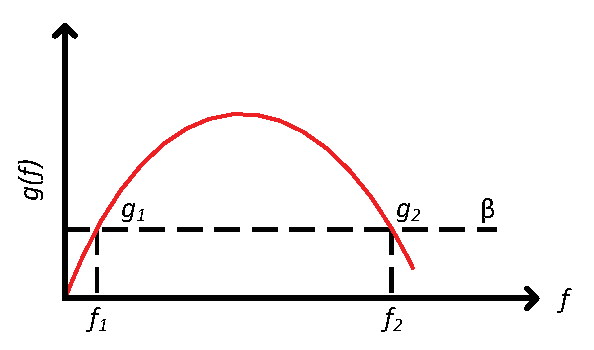
\includegraphics[width=0.8\linewidth]{fig/concave.eps}
\caption{Figure of PPW against clock frequency.}
\label{fig:concave}
\end{figure}
\section{PROOF OF QUASICONCAVITY OF PPW W.R.T. CLOCK FREQUENCY}
Let $g(f) = \frac{\left \| f \right \|_{1}}{\left \| P \right \|_{1}}$ be the PPW objective at some control cycle. $g$ is \emph{quasiconcave} iff its domain (\textbf{dom}) and all its super level sets $\mathit{S_{\beta}} = {f \in \textbf{dom } g~|~g(f)\geq \beta}$ are convex. 

Consider an ordinate $\beta$, which intersect the function $g$ at two points $(f_{1},g_{1})$ and $(f_{2},g_{2})$ as shown in Fig.~\ref{fig:concave}. We need to prove that the function between the two points is greater than or equal to $\beta$, i.e.
\begin{equation}\label{eq:ppw_transient_1}
g(\epsilon f_{1}+(1-\epsilon)f_{2})\geq \beta,
\end{equation}
where $\epsilon \in [0,1]$. $\beta$ can also be written as $\epsilon \frac{\left \| f_{1} \right \|_{1}}{\left \| P_{1} \right \|_{1}}+(1-\epsilon) (\frac{\left \| f_{2} \right \|_{1}}{\left \| P_{2} \right \|_{1}})$. And \eqref{eq:ppw_transient_1} can be written as
\begin{equation}\label{eq:ppw_transient_2}
\frac{\epsilon \left \| f_{1} \right \|_{1}+(1-\epsilon)\left \| f_{2} \right \|_{1}}{\left \|P(\epsilon f_{1}+(1-\epsilon)f_{2})\right \|_{1}} \geq \epsilon \frac{\left \| f_{1} \right \|_{1}}{\left \| P_{1} \right \|_{1}}+(1-\epsilon) (\frac{\left \| f_{2} \right \|_{1}}{\left \| P_{2} \right \|_{1}}).
\end{equation}
Let $P_{\epsilon}=P(\epsilon f_{1}+(1-\epsilon)f_{2})$, then \eqref{eq:ppw_transient_2} can be simplified to
\begin{equation}\label{eq:ppw_transient_3}
\epsilon\frac{\left \| f_{1} \right \|_{1}}{\left \| P_{1} \right \|_{1}}(\left \|P_{\epsilon}\right \|_{1}-\left \|P_{1}\right \|_{1})\leq(1-\epsilon)\frac{\left \| f_{2} \right \|_{1}}{\left \| P_{2} \right \|_{1}}(\left \|P_{2}\right \|_{1}-\left \|P_{\epsilon}\right \|_{1}).
\end{equation}
Since $\frac{\left \| f_{1} \right \|_{1}}{\left \| P_{1} \right \|_{1}}=\frac{\left \| f_{2} \right \|_{1}}{\left \| P_{2} \right \|_{1}}=\beta$, the above equation reduces to
\begin{equation}\label{eq:ppw_transient_4}
\left \|P_{\epsilon}\right \|_{1} \leq \epsilon \left \| P_{1} \right \|_{1}+(1-\epsilon)\left \| P_{2} \right \|_{1}.
\end{equation}
The above equation is a sufficient condition on convexity of $\left \| P \right \|_{1}$. It was shown in Appendix A that $P$ is convex w.r.t $f$. $\left \| P \right \|_{1}$ is the sum of elements in $P$. Therefore, $\left \| P \right \|_{1}$ is also a convex function w.r.t $f$. Hence, \eqref{eq:ppw_transient_4} is true and $g$ is a quasiconcave function of $f$.
\end{appendices}